\documentclass[tikz,border=8pt]{standalone}
\usepackage{tikz}
\usepackage{pgfplots}
\usepackage{amsmath,amssymb}
\usepackage[T1]{fontenc}
\usepackage{lmodern}
\usepackage{xcolor}
\usetikzlibrary{arrows.meta,positioning,shapes.geometric,fit,calc,backgrounds,matrix}
\pgfplotsset{compat=1.18}
\definecolor{ink}{HTML}{18202A}
\definecolor{blue}{HTML}{2563EB}
\definecolor{bluefill}{HTML}{EAF1FF}
\definecolor{green}{HTML}{14804A}
\definecolor{greenfill}{HTML}{E8F6EE}
\definecolor{amber}{HTML}{B56A00}
\definecolor{amberfill}{HTML}{FFF3D6}
\definecolor{red}{HTML}{B42318}
\definecolor{redfill}{HTML}{FDECEC}
\definecolor{gray}{HTML}{667085}
\definecolor{light}{HTML}{F4F6F8}
\definecolor{linegray}{HTML}{C7CDD4}
\tikzset{
  box/.style={draw=ink, rounded corners=3pt, very thick, fill=white, align=center, inner sep=7pt, font=\sffamily\small},
  bluebox/.style={box, fill=bluefill, draw=blue},
  greenbox/.style={box, fill=greenfill, draw=green},
  amberbox/.style={box, fill=amberfill, draw=amber},
  redbox/.style={box, fill=redfill, draw=red},
  ghost/.style={draw=linegray, rounded corners=3pt, thick, fill=light, align=center, inner sep=7pt, font=\sffamily\small},
  label/.style={font=\sffamily\footnotesize, text=gray, align=center},
  title/.style={font=\sffamily\bfseries\large, text=ink, align=center},
  arrow/.style={-{Latex[length=3mm,width=2mm]}, very thick, draw=ink},
  bluearrow/.style={-{Latex[length=3mm,width=2mm]}, very thick, draw=blue},
  redarrow/.style={-{Latex[length=3mm,width=2mm]}, very thick, draw=red},
  greenarrow/.style={-{Latex[length=3mm,width=2mm]}, very thick, draw=green}
}

\begin{document}
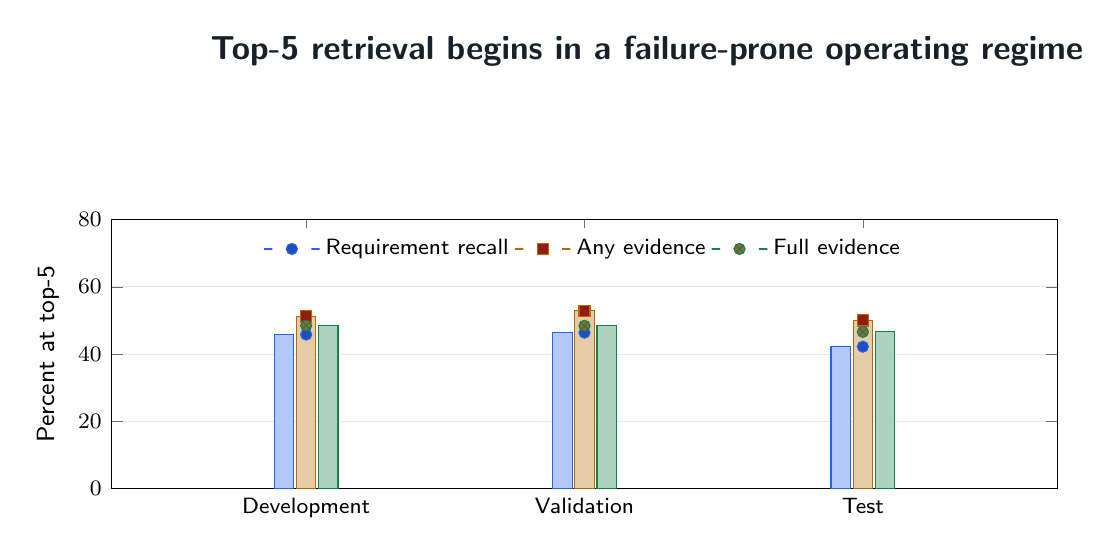
\begin{tikzpicture}
\node[title] at (7.4,5.9) {Top-5 retrieval begins in a failure-prone operating regime};
\begin{axis}[
 at={(0.6cm,0.35cm)}, anchor=south west,
 width=13.6cm,height=5.0cm,
 ymin=0,ymax=80, xmin=0.3,xmax=3.7,
 xtick={1,2,3}, xticklabels={Development,Validation,Test},
 ylabel={Percent at top-5},
 ymajorgrids=true, grid style={draw=linegray!45},
 legend style={at={(0.5,0.97)},anchor=north,legend columns=3,draw=none,font=\sffamily\footnotesize,fill=white},
 tick label style={font=\sffamily\footnotesize}, label style={font=\sffamily\small},
]
\addplot+[ybar,bar width=7pt,bar shift=-8pt,fill=blue!35,draw=blue] coordinates {(1,45.80)(2,46.37)(3,42.20)};
\addplot+[ybar,bar width=7pt,bar shift=0pt,fill=amber!35,draw=amber] coordinates {(1,51.19)(2,52.88)(3,50.00)};
\addplot+[ybar,bar width=7pt,bar shift=8pt,fill=green!35,draw=green] coordinates {(1,48.49)(2,48.40)(3,46.60)};
\legend{Requirement recall,Any evidence,Full evidence}
\end{axis}
\end{tikzpicture}
\end{document}
